
% This template has been edited from the IEEE template available at:
% https://www.ieee.org/conferences/publishing/templates.html
%
% For further help, you may wish to see:#
% https://www.overleaf.com/learn/latex/tables
% https://www.overleaf.com/learn/latex/Inserting_Images
% https://www.overleaf.com/blog/532-creating-and-managing-bibliographies-with-bibtex-on-overleaf

\documentclass[conference]{IEEEtran}
%\IEEEoverridecommandlockouts
% The preceding line is only needed to identify funding in the first footnote. If that is unneeded, please comment it out.
\usepackage[a4paper, total={6in, 8in}, margin=0.75in]{geometry}
\usepackage{cite}
\usepackage{amsmath,amssymb,amsfonts}
\usepackage{algorithm} 
\usepackage{algpseudocode} 
\usepackage{graphicx}
\usepackage{textcomp}
\usepackage{xcolor}
\usepackage{color,soul}
\usepackage{float} % to allow figures across 2 columns

\def\BibTeX{{\rm B\kern-.05em{\sc i\kern-.025em b}\kern-.08em
    T\kern-.1667em\lower.7ex\hbox{E}\kern-.125em}}
\begin{document}

\title{Achieving Accurate Odometry Through Self-Calibration - A Robot's Quest to Find Itself}

\author{
    \IEEEauthorblockN{xq19351}
    \and
    \IEEEauthorblockN{xl19540}
}

\maketitle

\begin{abstract}
It is normal to write the abstract last.  First, try to concisely state the problem/question/challenge under investigation.  Second, state what you found out.  The abstract should help a reader decide if they are interested in reading the whole paper.  Keep your abstract short.  Don't rely on the abstract to introduce your work.
\end{abstract}


\section{Introduction}\label{sec:intro}

The use of mobile robotics in industry is becoming more common for logistics, deliveries and manufacturing
One of the key challenges when deploying autonomous mobile robots is accurate odometry, which is the process of using sensor data and robot kinematics to calculate the position of the robot over time.
Industrial robot accuracy requires a detailed understanding of a robot's dimensions,
Slight variations in dimensions due to manufacturing tolerances require individual calibration for each robot to be accurate.
This is often achieved through manual calibration, a slow process that is prone to user error and impractical for large swarms of robots. 

Accurate odometry aims to reduce systematic errors, caused by inaccuracies in robot dimensions, sensors or actuators. Non-systematic errors are random errors that are caused by variation in the robot's environment and are generally less critical as they do not accumulate over time.
Generally the radius and wheelbase error are reflected in literature as the most common sources odometry error \cite{UMBmark, width-radius}.

Automatic calibration through a pre-determined test circuit, can be used to measure the robots key dimensions and set up accurate kinematic for each robot. This reduces human error and speeds up the process.

This report develops an automatic calibration circuit and method to measure the key dimensions of a Polulu 3Pi+ robot using its onboard sensors and processors, aiming to reduce the need for time-consuming manual adjustments. This should minimise systematic errors \cite{odometry} 

The 3Pi+ is a robot designed for learning and as such is manufactured cost-effectively meaning that component tolerances and sizing can vary. As a result, well-programmed robots will produce precise but potentially inaccurate results when tested for tasks that require accurately angled or distanced movements. 

\begin{figure}[h!]
    \centering
    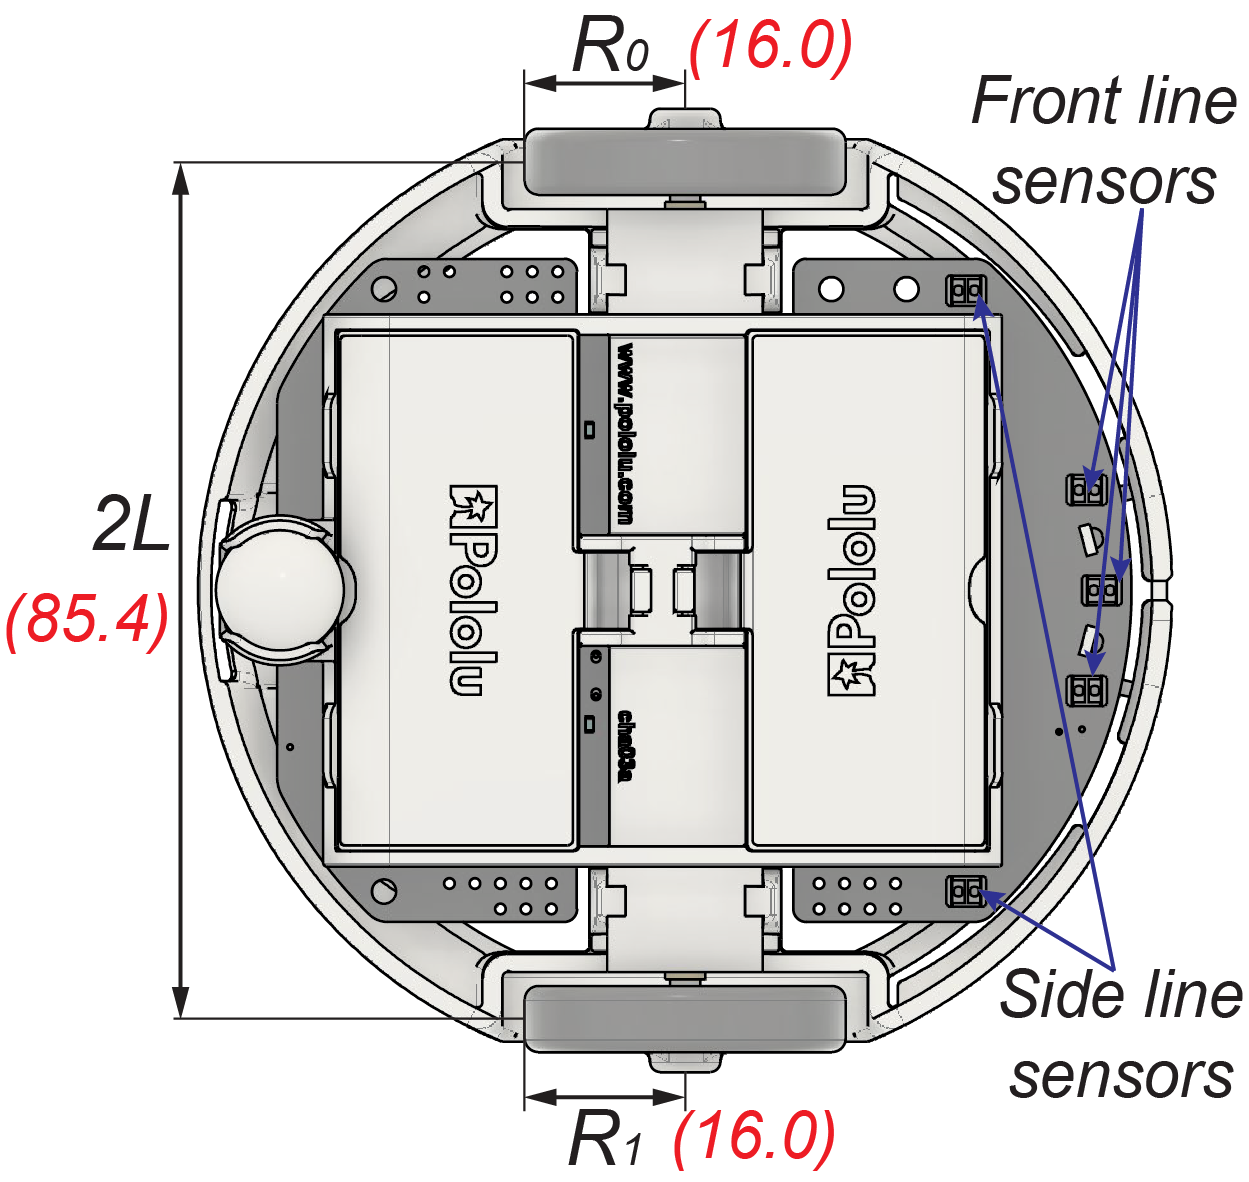
\includegraphics[width = 0.49\textwidth]{img/robot_schemtatic.png}
    \caption{Bottom view of the Pololu 3Pi+ CAD model with dimensions \cite{pololu_guide}}
    \label{fig:dimensions}
\end{figure}

Among the 3Pi+'s extensive range of sensors, the robot contains wheel encoders and infrared-radiation (IR) sensors \cite{pololu_guide}. 

The two key dimensions used in the differential drive kinematics model are the width of the wheelbase and the wheel diameters \cite{pololu_guide}, shown in Figure \ref{fig:dimensions}.


\subsection{Hypothesis Statement}

As part of this study, there are two key hypotheses related to robot calibration. The first is that individual robots require individual calibration to achieve the same odometry accuracy. The second hypothesis is that individual calibration can be achieved through an automatic one-time offline calibration using a calibration circuit.

\begin{quote}
    \emph{
    The authors hypothesize that variances in wheel diameter and wheelbase width significantly affect the odometry accuracy of the Pololu 3Pi+ robot.
    This experiment predicts that a calibration circuit and method using onboard sensors can automatically measure key robot dimensions in the kinematic model.
    By applying this calibration, we anticipate a measurable improvement in accuracy through a reduction in systematic odometry errors, when compared to performance using default dimensions.
    }
\end{quote}


% These hypothesese will be tested by two accuracy tests on the robot. 
% The hypothesis will be enacted by creating a calibration code that works on a predefined test circuit, and then the robot is tested using both the UMBmark test and a straight line distance. 
% The first test will confirm the heading angle (theta) error and the second will confirm a distance error. 
% If both of these tests indicate a better performance after calibration then the hypothesis will be accepted.

% By minimising the human interaction required this process can be made quicker and cheaper, hence the use of automated measurements on a pre-designed circuit.


\section{Implementation}\label{sec:implementation}

The system's odometry accuracy is evaluated using two tests: linear distance and orientation angle. 
Initially, these tests were conducted on the uncalibrated system, using the default dimensions provided in the 3Pi+’s datasheet for the kinematic model. This establishes a baseline for performance.

Next, the robot was run on a printed calibration test circuit, using line sensor feedback to determine robot-specific dimensions. 
These dimensions are updated in the kinematic model and the calibrated system is retested to determine if there is an improvement in odometry accuracy.

\paragraph{Linear accuracy} The linear accuracy is tested by measuring a known distance using the 3Pi+'s line sensors and comparing the measured value to the true distance.
The robot is driven at a slow, constant speed across two marked points spaced 500mm apart.
The robot records the number of wheel rotations between the tick marks (N), measured by the encoders, and calculates the distance travelled using:

\begin{equation}
    D = 2 \pi R N
\end{equation}

The distance measurement is taken between the two rising edges of the line sensor's detection signal, shown in Figure \ref{fig:linesensor}.
This aims to minimise any variation in distance measurements caused by changes in ambient light, which affects how early the sensor line detection threshold is crossed.

\begin{figure}[h!]
    \centering
    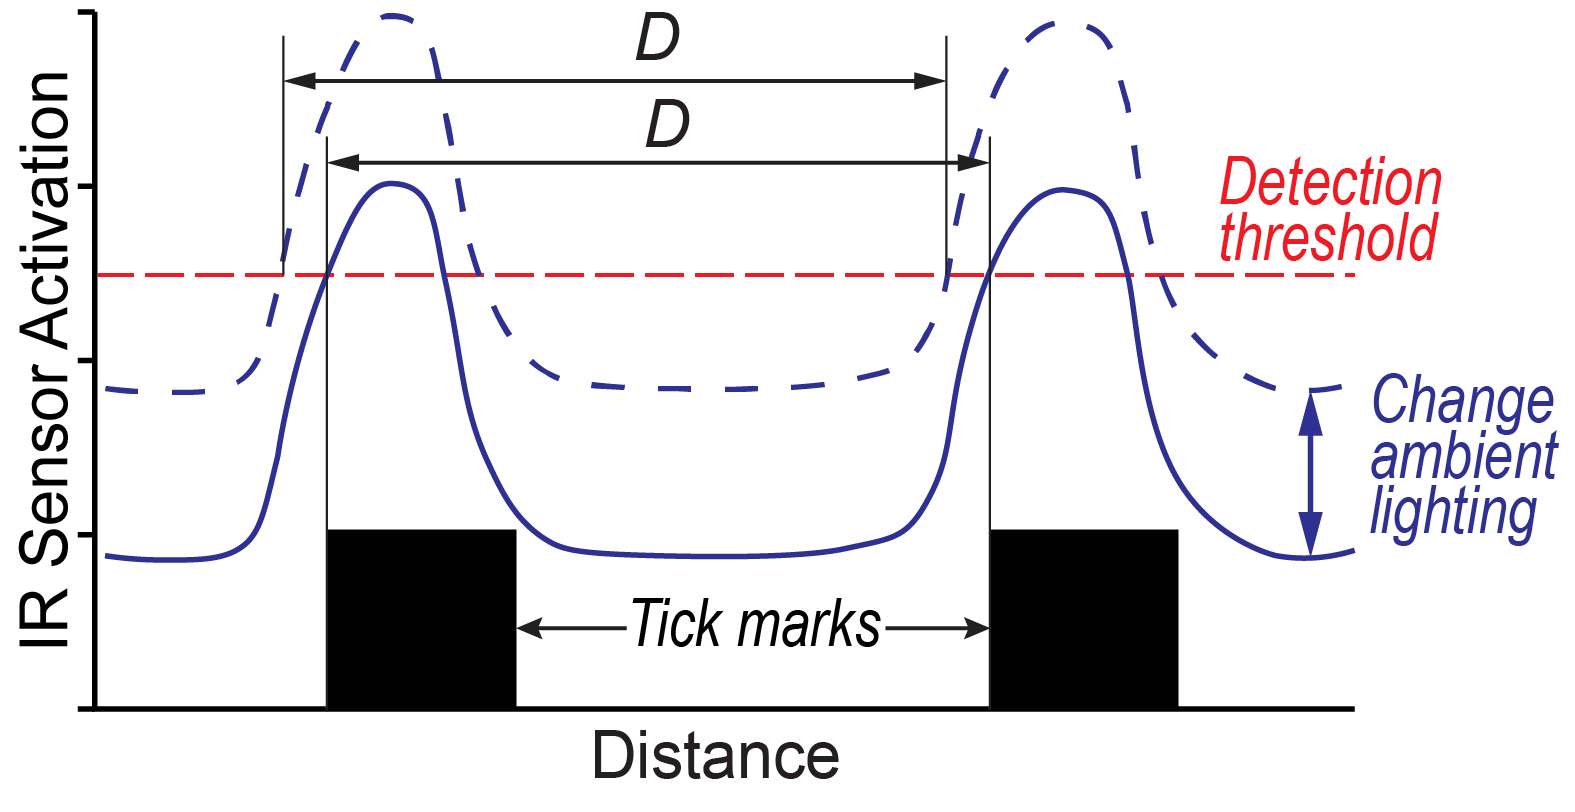
\includegraphics[width = 0.47\textwidth]{img/linesensor_response.png}
    \caption{Line sensor response and activation threshold}
    \label{fig:linesensor}
\end{figure}

\paragraph{Orientation accuracy}
The orientation accuracy of the robot is measured using the UMBmark test \cite{UMBmark}. 
The robots complete two circuits around a 0.5m square and the orientation and distance error from the origin are recorded.
Driving around the square twice, amplifies the accumulated systematic error, making it easier to measure precisely. 
The test is run both clockwise and anti-clockwise to distinguish between systematic errors that cancel each other out.

\paragraph{Calibration}
A test circuit was designed to calibrate the 3Pi+’s kinematics, shown in Figure \ref{}. 
The line sensors are used to control the movement of the robot along the pre-defined printed path, allowing the deviation between the kinematic model and the true circuit dimensions to be used to calculate the wheel radii and the wheelbase length.

\begin{figure}[h!]
    \centering
    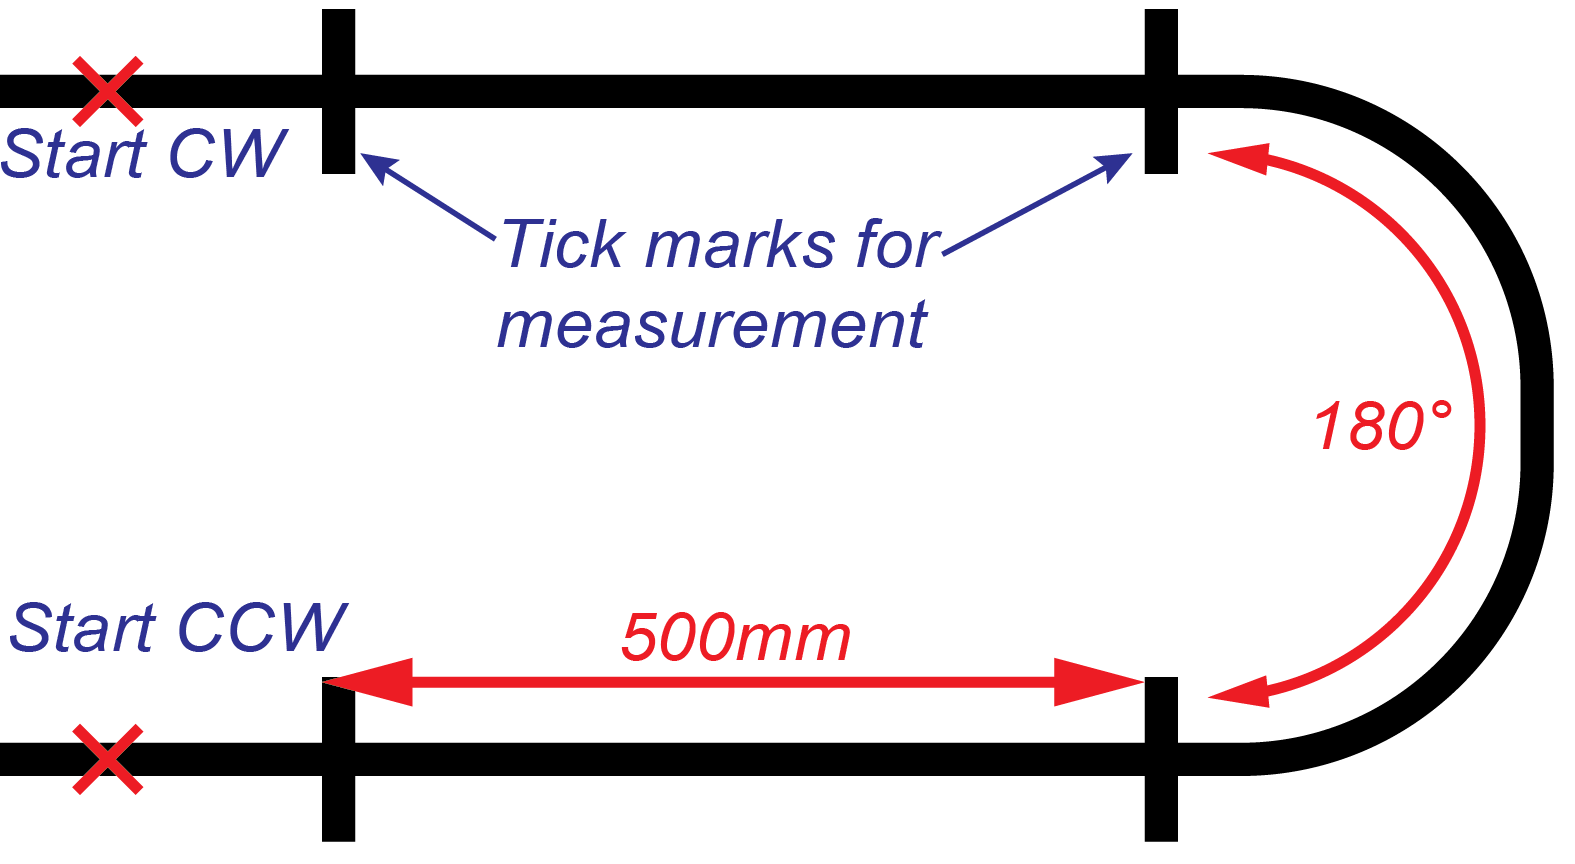
\includegraphics[width = 0.49\textwidth]{img/calibration_circuit.png}
    \caption{Circuit diagram}
    \label{fig:calibration_circuit}
\end{figure}

The circuit comprises of a 0.5m straight line section, followed by a 180 degree turn, followed by another 0.5m straight line section. 
At the beginning and end of each section a perpendicular tick mark is printed to be used for the calibration procedure. 
It is symmetrical to ensure that any calibration differences between a clockwise and anticlockwise calibration are averaged out.

\hl{needs a bit of re-wording:}
The robot will complete the circuit by using the front line sensors to follow the path. 
The side line sensors are used to begin and end the calibration calculations. 
First, the robot completes the straight line section, measuring the distance between the tags based on the internal kinematics, comparing this to the known distance to calculate the wheel radii as seen in equation \ref{eq:linear}. in equations \ref{eq:linear} and \ref{eq:angle}, $R_i$ are the radii of the wheels, $C$ is the number of encoder counts per revolution, $d,\alpha$ are the circuit parameters: straight line distance and turn angle and $e_i$ are encoder counts for each wheel.

\begin{equation}
\label{eq:linear}
    R_i = \frac{C \times d}{2 \times \pi \times \Delta e_i}
\end{equation}

The robot then completes the turning section of the circuit, measuring the turn angle based on internal kinematics and comparing this to the known turn angle to calculate, with updated wheel radii, the wheelbase length $L$, as seen in equation \ref{eq:angle}.

\begin{equation}
\label{eq:angle}
L = \left|\frac{\pi \times (\Delta e_0 \times R_0 - \Delta e_1 \times R_1)}{\alpha \times C}\right|
\end{equation}

Upon completion, the robot will enter a state in which it repeatedly prints these new values to the serial monitor. These values will then be updated manually in the kinematics of that robot.


% \begin{algorithm}

% \caption{Calibration Method} 
%     \label{algo:calibration}
% \textbf{Input:} Line sensor readings left to right:  linesensor[0,1,2,3,4], known length \textbf{and} angle \\
%  \textbf{Output:} Array of dimensions, $R_0,R_1,L$\\

%     \begin{algorithmic}
%         \State State = 1
        
%         \State \textbf{Update state:}
%         \If{State = 1
%         \textbf{and} linesensor[0] \textbf{and} linesensor[4]}
%             \State State = 2
%         \ElsIf{State = 2 \textbf{and} \textbf{not} linesensor[0] \textbf{and} \textbf{not} linesensor[4]}
%             \State Update encoder counts
%             \State State = 3
%         \ElsIf{State = 3 \textbf{and} linesensor[0] \textbf{and} linesensor[4]}
%             \State Calculate $R_0, R_1$ \textbf{or} $L$ 
%             \State State = 4
%         \EndIf\\
        
%         \State \textbf{State Actions:}
%         \If{State = 1 \textbf{or} State = 2 \textbf{or} State = 3}
%             \State Follow line
%         \ElsIf{State = 4}
%             \State Stop motors
%             \State Print $R_0,R_1,L$
%         \EndIf
%     \end{algorithmic}
% \end{algorithm}

\section{Experiment Methodology}\label{sec:experiment_method}

% \begin{itemize}
%     \item Run baseline accuracy tests for a number of robots. (linear distance and square error)
%     \item Run the calibration procedure to identify new dimensions for the robot.
%     \item Test the calibrated robots on the same set of accuracy tests.
%     \item Identify if there is an improvement.
% \end{itemize}

\subsection{Overview of Method}

The baseline, calibration and post-calibration tests were conducted on 3 different robots to investigate the variation between robots. 

First, the linear and orientation tests are completed on un-calibrated robots (using the default dimensions found on the robot data sheet \cite{}) to establish a baseline set of results. 
The linear distance test is run ten times for each robot, documenting the error on each run. 
The orientation test involves two laps around the square track, completed five times in each direction; clockwise and anti-clockwise.
Both orientation and position error from the origin are recorded.

Each robot is then calibrated using the calibration circuit and calibration algorithm. 
The resulting measured robot dimensions from 10 repeat calibrations are recorded (for 5 in each direction).
The calibrated mean values for each wheel radius and wheelbase length are updated for each of the robot's kinematic models. 

Finally, each robot is re-tested on the original linear and orientation error tests in an identical manner to the baseline tests. 

\subsection{Discussion of Variables}

\begin{itemize}
    \item \textbf{Controlled Variables}: 
    For each test, the \emph{distance} and number of \emph{laps} are kept constant. 
    Each robot runs the same test code, using the same kinematic model, motor and heading PID controllers. 
    Furthermore, \emph{ambient lighting} is kept constant due to its influence on the readings from the IR line sensors. 
    New, fully charged batteries are used for each set of tests.
    \item \textbf{Independent Variable}: 
    The independent variable is the robot itself. 
    
    
    As the experiment relies on autonomous measurement by the robot, the only changing variable will be the robot, and as a result the robot dimensions - $R_0, R_1, L$. 
    The method aims to observe a measurable difference in these parameters between robots and use this to explain any improvements in system accuracy after calibration. 
    \item \textbf{Dependent Variable(s)}: this experiment aims to measure the accuracy of the robots before and after calibration. The metrics used for quantifying the accuracy are the linear error for linear tests, orientation error and Euclidean distance error on return-to-home on the orientation test.
\end{itemize}

identical differential drive kinematics model and tuned PID control of the motor speed and robot heading must be used. 
The speed and acceleration of the robots is limited to avoid wheel slippage.

\subsection{Discussion of Metric(s)}

The calibration process aims to change:
\begin{enumerate}
    \item the radii of the wheels,
    \item the width of the wheelbase,
\end{enumerate}
for each robot from the default values found in the data sheet.

The outcomes on the following variables will be measured to quantify the results:
\begin{enumerate}
    \item Linear error and p-value for error change
    \item Orientation error and p-value for error change
    \item Absolute position error and p-value for error change
\end{enumerate}

The linear error is used as it demonstrates the error from overshoot (positive error) and undershoot (negative error) due to incorrect wheel radius values $R_0, R_1$. This metric is isolates the impact of wheel radii as the test is conducted on a straight line section and the wheelbase length $L$ does not impact the result, as seen in equation \ref{eq:linear}.

The orientation error is quantified with the error in angle on return to the origin. This error is an accumulation of the orientation errors during the test meaning that this metric provides an estimate of the systematic orientation error.
The orientation error, given correct wheel radii (as found in the first part of the calibration), isolates the impact of the wheelbase width $L$ allowing this metric to measure the effect of that variable on robot accuracy.

Finally, the Euclidean position error encompasses an overall odometry systematic error found for each robot. This provides an overall measure of robot accuracy and precision. The spread of error corresponds to the overall precision and the mean values correspond to the overall accuracy. 
This metric and both of these observations provide a clear comparison point for robot performance before and after calibration.


\section{Results}\label{sec:results}


The results of the tests before and after calibration are shown in the section, comparing the change in metrics for each of three robots. 
A paired t-test has been used to assess the significance of the results for each robot. A paired t-Test is selected as the variance of results before and after calibration is not assumed to be equal as this could be impacted by the calibration. The tests are performed at a 5\% significance level.

\subsection{Measured dimensions}

The dimensions measured by the calibration method for each of the three test robots are shown in Figure \ref{fig:r0r1L}. Although measurable, the difference between dimensions (R0, R1 and L) of any of the robots is not statistically significant \hl{($n = 10$, two-tail, $p > 0.05 $)} for any pairing. The median wheel radius is 16.25mm rather than 16mm. Similarly, the median wheelbase is 42.87mm rather than 42.7mm.

\begin{figure}[h]
    \centering
    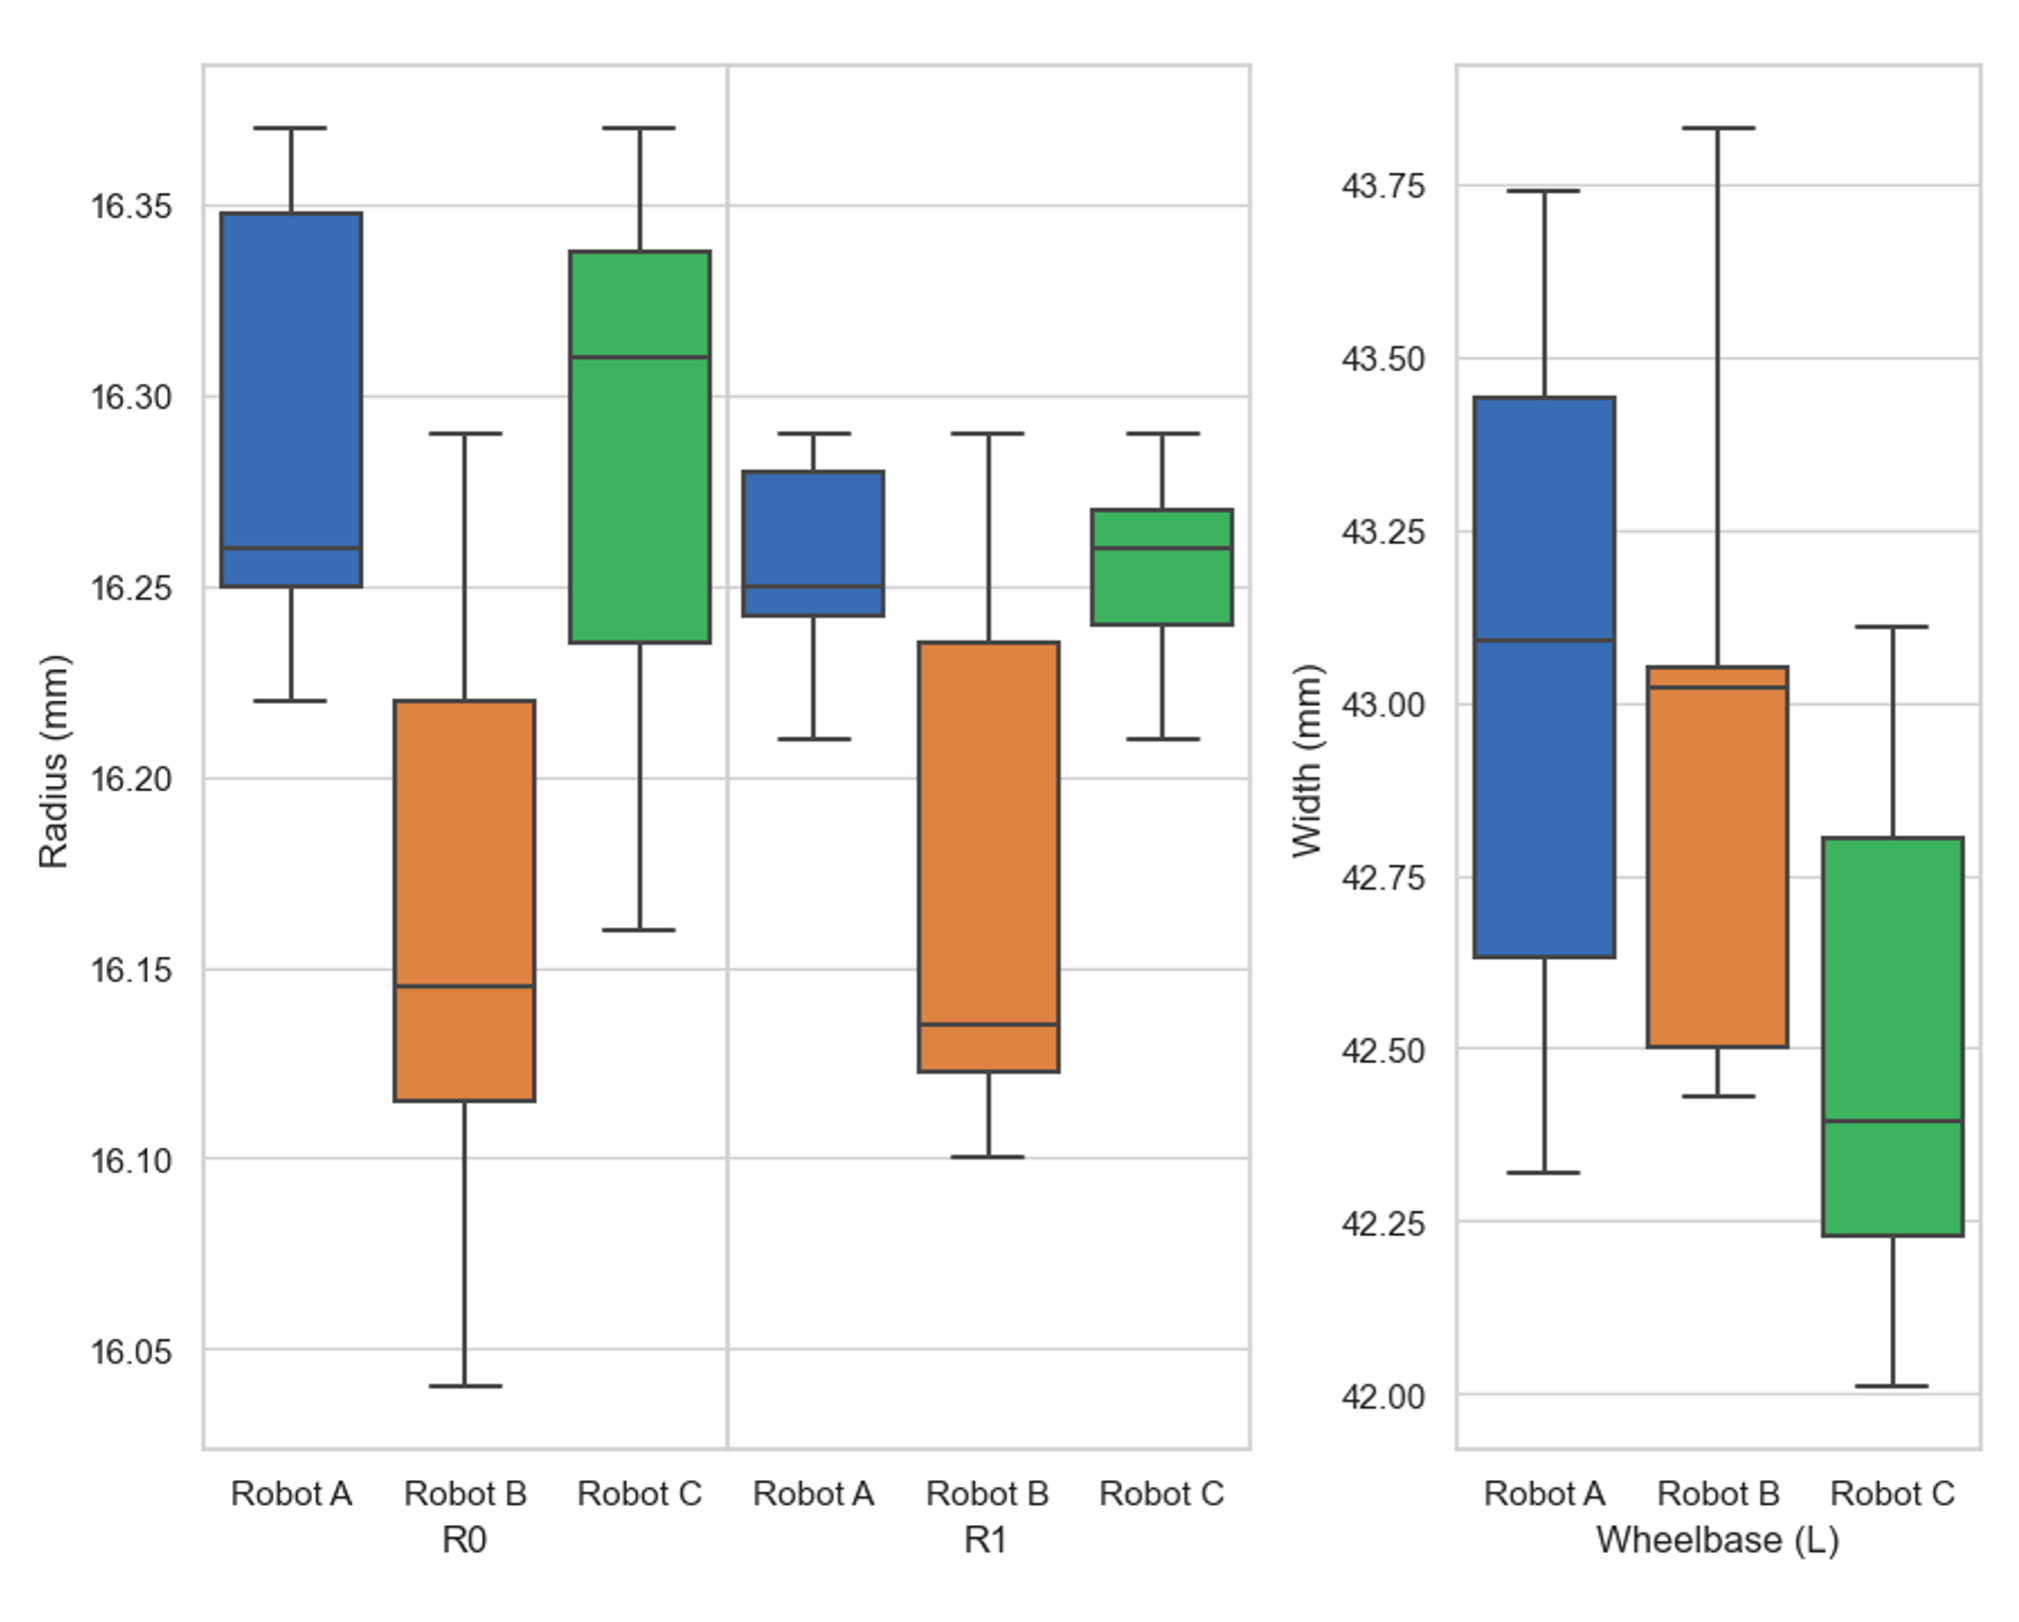
\includegraphics[width=.5\textwidth]{img/r0r1l.png}
    \caption{Measured key dimensions}
    \label{fig:r0r1L}
\end{figure}

\subsection{Linear accuracy}

The first test compared results of the linear accuracy measurement of the three robots. 
Pre-calibration the three robots all undershoot by varying amounts, while post-calibration the robots' absolute mean error is smaller by an average of 8.2mm, showing a statistically significant decrease in error with an average paired t-test ($n = 10$, one-tail, $p = 0.004$). The distribution of errors for the three robots is shown in Figure \ref{fig:linear}.

\begin{figure}[h]
    \centering
    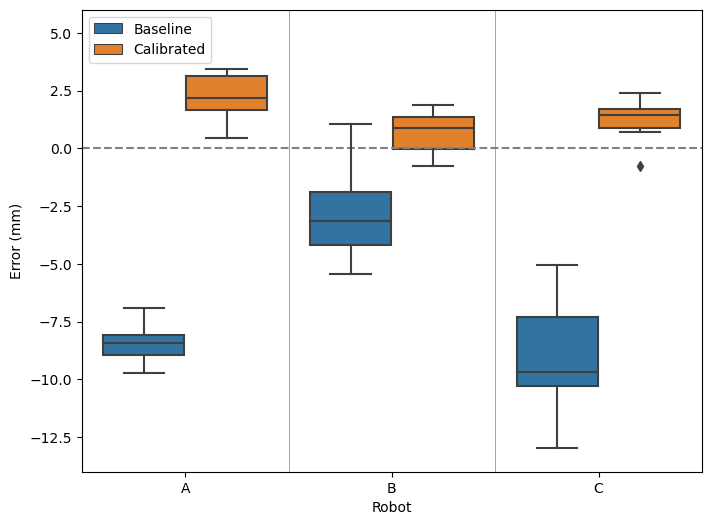
\includegraphics[width=.45\textwidth]{img/linear_pre_post.png}
    \caption{Linear error over 500mm before and after calibration}
    \label{fig:linear}
\end{figure}

\subsection{Orientation accuracy}

The orientation error calculated from the UMBmark test is plotted in Figure \ref{fig:orientation}. The distributions appear to show a clustering of results based on the direction of travel around the test circuit in the baseline results.

\begin{figure*}[h!]
    \centering
    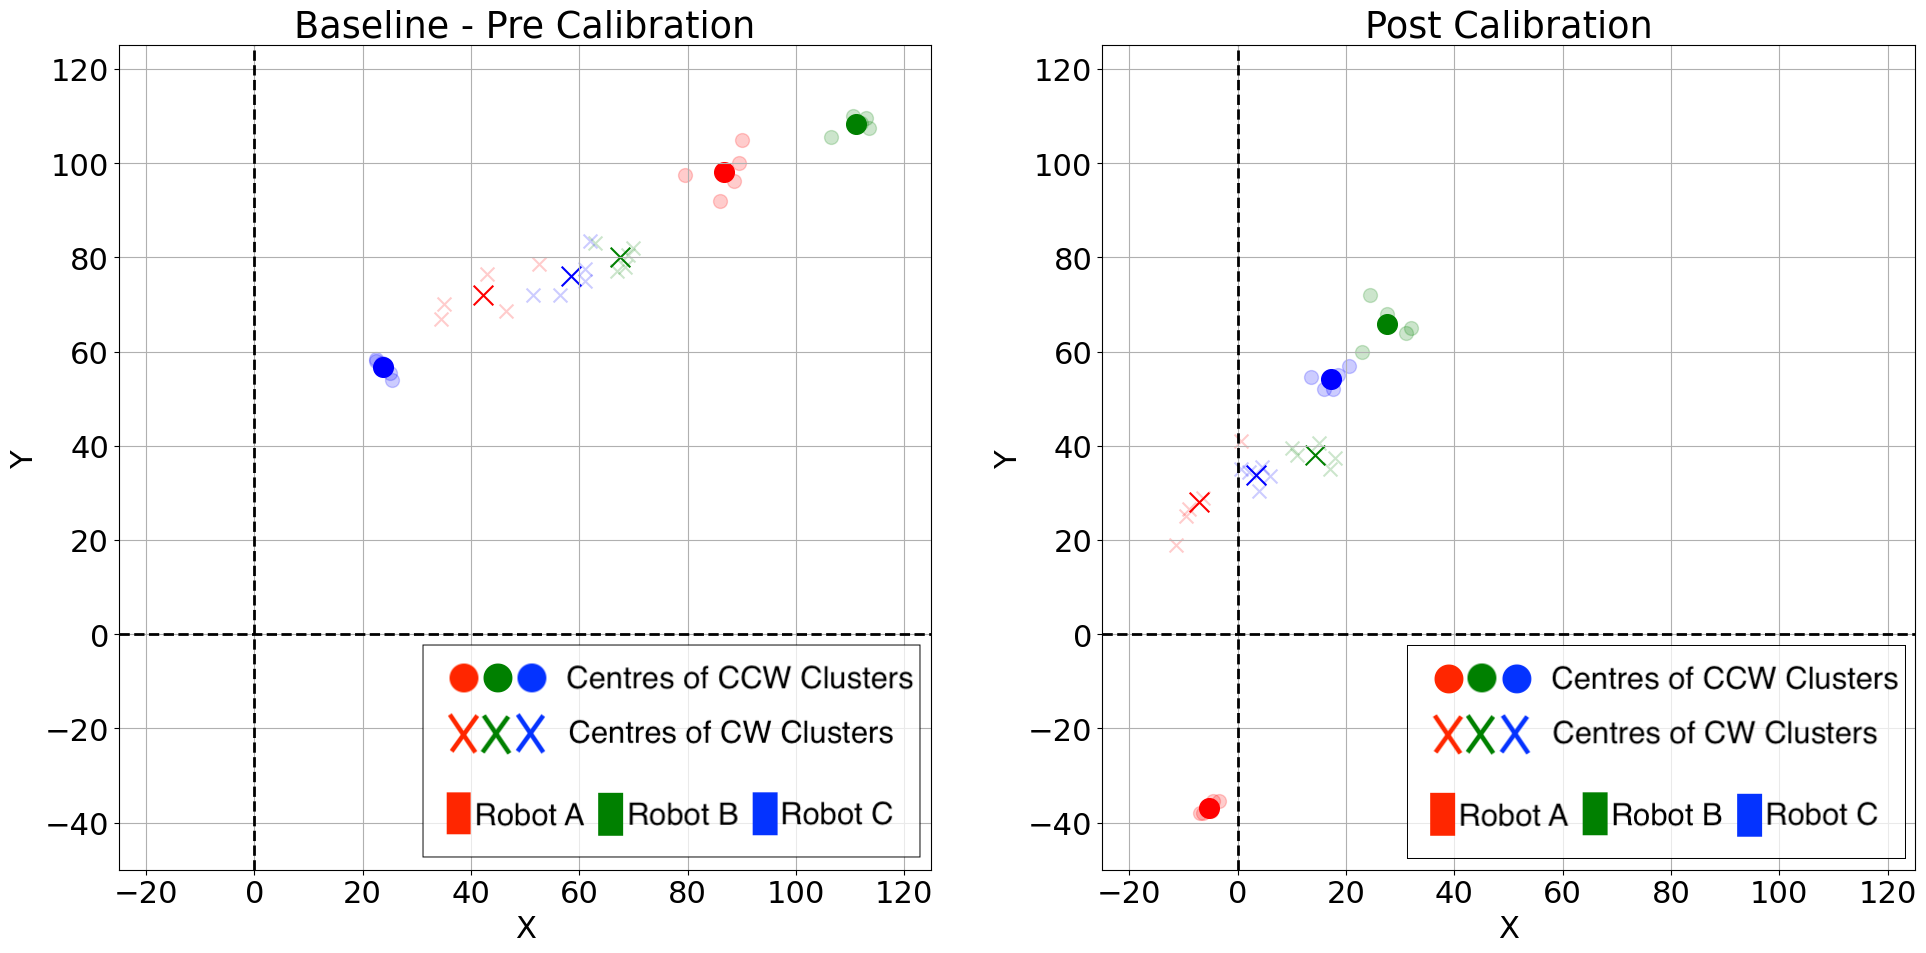
\includegraphics[width=.9\textwidth]{img/xy_pre_post_2.png}
    \caption{Return to home position relative to the origin for all three robots in the clockwise and anticlockwise direction. The darker marks show the mean location for each cluster.}
    \label{fig:xy_scatter}
\end{figure*}

\begin{figure}[h!]
    \centering
    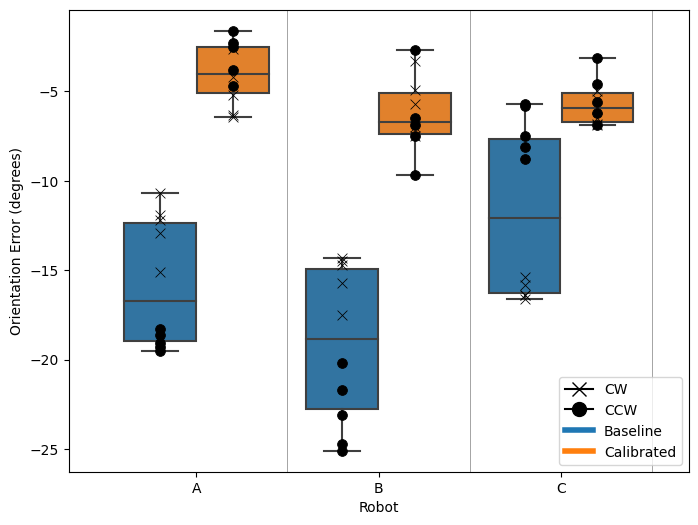
\includegraphics[width=.45\textwidth]{img/orientation_error.png}
    \caption{Orientation error before and after calibration}
    \label{fig:orientation}
\end{figure}



A paired t-test reveals that there is significant clustering ($n = 5$, one-tail, $p < 0.05$) for all robot test results apart from the post-calibration result of Robot A ($p=0.051$). The test also reveals an average increase in p-value between pre-calibration and post-calibration of over two orders of magnitude (143.9) suggesting that the clustering reduces as a result of calibration. 

Additionally, Figure \ref{fig:orientation} shows a reduction in orientation error between the baseline and calibrated measurements for all robots. The difference is statistically significant ($n = 10$, one-tail, $p < 0.05$) for all robots with p-values $p=1.5\times10^{-6}$, $p=2.9\times10^{-9}$ and $p=0.01$ respectively. 

\begin{figure}[h!]
    \centering
    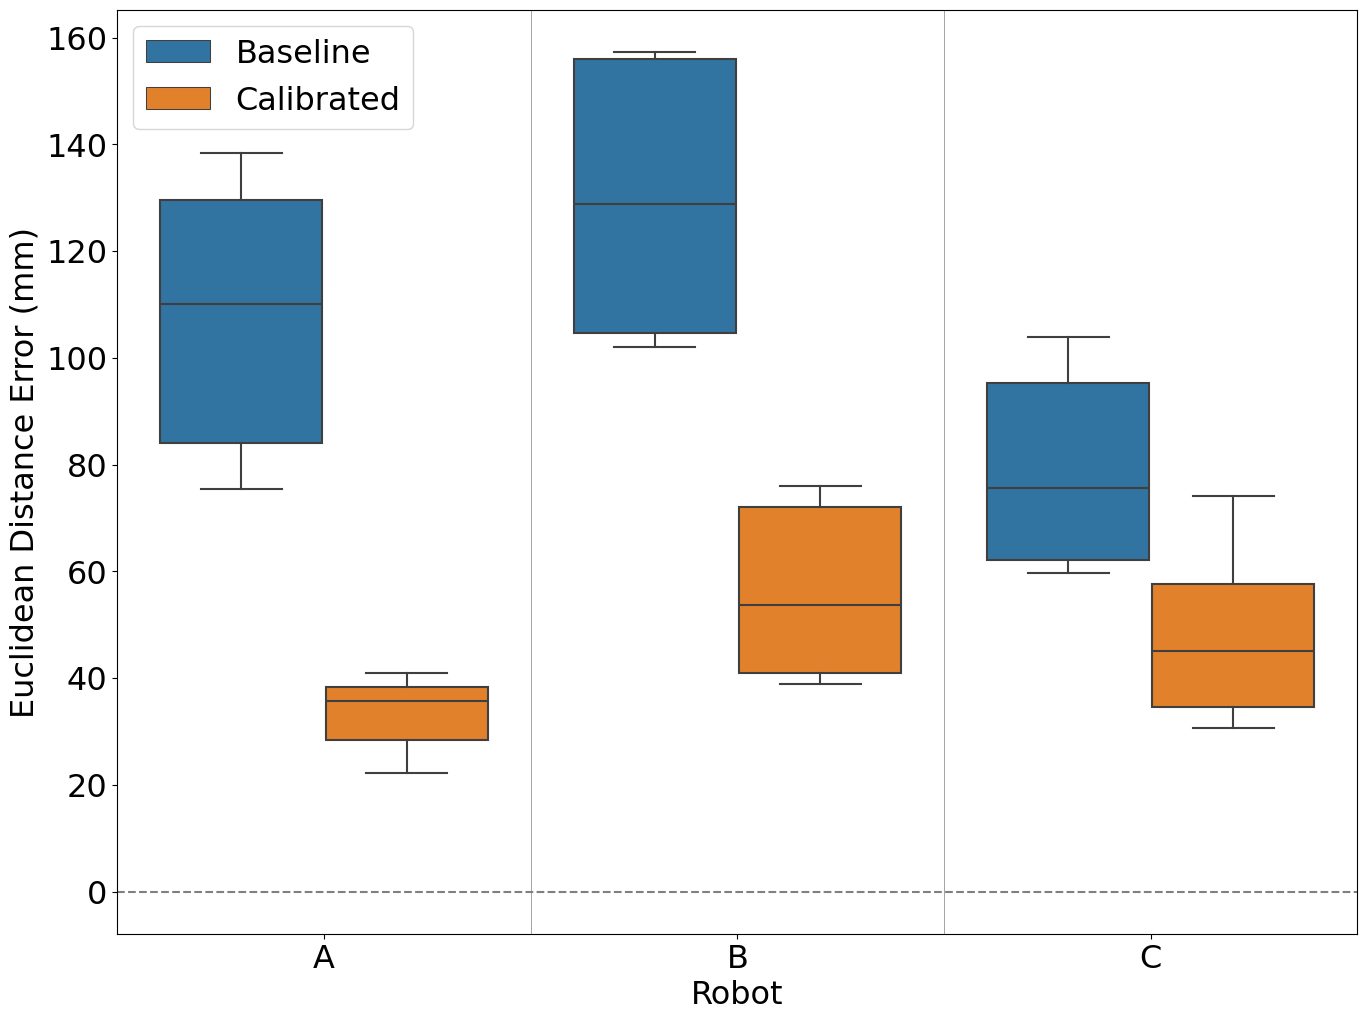
\includegraphics[width = 0.45\textwidth]{img/xy_error_boxplot.png}
    \caption{The Euclidean distance error in return to home position before and after calibration.}
    \label{fig:xy_box}
\end{figure}

Figures \ref{fig:xy_scatter} and \ref{fig:xy_box} show the pre and post-calibration position error from the UMBmark tests. 
The cluster centres are marked and separated by the test direction (CW or CCW).
Figure \ref{fig:xy_box} shows the distribution of linear Euclidean distances from the origin at the end of UMBmark tests, indicating a decrease in position error and standard deviation of errors. 
The average standard deviation was reduced by 10mm to 14mm after calibration.
For all robots, the return to home error paired t-test found the difference between means to be significant ($n = 10$, one-tail $p < 0.05$). 

\section{Discussion and Conclusion}\label{sec:discussion_conclusion}

The results of this study are used to discuss the original hypothesis:

% Make a discussion of what your results showed - whether this supported or refuted your hypothesis. Try not to respond to your hypothesis as if you were right or wrong, or successful or unsuccessful.  Instead, evaluate your hypothesis for whether it helped you to learn something - was it a good question or prediction to make?  Was it useful in this way?  If not, in what way does the hypothesis need adjustment, to guide future experiments? 
% In your discussion, use this as another opportunity to demonstrate/evidence your understanding. Try to avoid stating the obvious - instead, use analysis/evaluation/synthesis to show that you understand \emph{how} and \emph{why} you saw the results you did. 



\begin{quote}
    \emph{
    The authors hypothesize that variances in wheel diameter and wheelbase width affect the odometry accuracy of the Pololu 3Pi+ robot.
    This experiment predicts that a calibration circuit and method using onboard sensors can automatically measure key robot dimensions.
    By applying this calibration, we anticipate a measurable improvement in accuracy through a reduction in systematic odometry errors, when compared to performance using default dimensions.
    }
\end{quote}

\paragraph{Meaning}
An overall analysis of the results suggests that there are measurable but not statistically significant differences in the key robot dimensions. 
This is not surprising given that size deviation would be measured during manufacturing, and statistically significant deviation would not pass quality control checks. 
Although the average deviation from the official dimensions is 1.5\% for the radii and 0.4\% for the wheel base, this deviation, particularly in the radius dimension is shown to be consistent between robots.
This suggests that setting the default radius value to 16.25mm rather than 16mm would likely improve the accuracy of most robots.

The hypothesis is further supported by evidence in the linear and orientation accuracy tests, suggesting that automatic calibration can improve the accuracy and precision of the robotic system. 

In order of results:
Linear error and standard deviation decrease as a result of calibration.
Orientation error and the difference between CW and CCW results decreases as a result of calibration.
The final position error decreases significantly and and the standard deviation also decreases.



But talk about the difference in directions.

Talk about the importance of the line sensor reading accuracy to this method




\paragraph{Limitations}

\hl{limitations}
The findings in this report are limited by a number of factors related to systematic and non-systematic errors and assumptions used for the control of the robot.

The differential drive kinematic model assumes that wheel revolutions are directly proportional to linear distance, neglecting wheel slippage and mechanical differences in the drive \cite{odometry}.

Additionally, the system makes use of a PID controller that has been tuned to only one robot. For repeatability, this report assumes a calibrated PID with the responses of such a controller likely differing between robots. 
To reduce the impact of a controller a larger test distance should be used, thereby allowing more time for a heading response to settle in the case of the UMBmark test.

The are a number of potential sources of systematic error that are assumed to be negligible in this investigation, these are the gearbox slip, misalignment of wheels and the limits of the encoder resolution. There is significant evidence in literature that the impact of these factors is much less than of those investigated in this study. However it is likely that these factors cause the differences between robot performance.



- gearbox slip
- you already need a calibrated a PID,tuned to only one robot
- battery
- wheel sizes are limited
- Relies on the accuracy of the printed calibration sheet
- Limits of the kinematic model - assumes linear movements does not calculate arcs or something like that




It is understood that other robot features may also vary between the robots: \hl{the gearbox backlash etc} however this report predicts that such difference result in a lower magnitude error in accuracy and as such will not impact the analysis of results.


\hl{further work:}
automation, ensure that the external features are accounted for better? - lighting and gearbox
counts per rev

% Use the Conclusion section to discuss the implications of your study.  This should therefore link back to your introduction, which began with a broad statement of the problem area.  Now, with your results providing evidence, you could attempt to make recommendations for applications in this area or for future studies.
% This is also a good opportunity to evaluate your experiment and project as a whole.  You may wish to further discuss the limitations of the study (e.g. the difficulty of controlled/dependent variables, or any problems you faced in your project).  When you did discover limitations in your method, use this to illustrate that you understand the issue by detailing how it could be rectified in future work.  When making a recommendation for future work ensure that this is a clear advancement from the understanding you have gained and not wild speculation.  It is not useful to see future work like ``I would use a high resolution doppler radar instead" - because this doesn't improve our understanding of your reported work, or how your work could be advanced in a meaningful way.




\bibliographystyle{ieeetr} 
\bibliography{biblio}


\end{document}
